\documentclass[10pt,a4paper]{article}
\usepackage[margin=20mm,headheight=14pt]{geometry}
\usepackage[T1]{fontenc}
\usepackage{lmodern,microtype}
\usepackage{xcolor,booktabs,array,tabularx}
\usepackage{xurl,hyperref,fancyhdr}
\usepackage{tikz}
\usetikzlibrary{arrows.meta,positioning}
\definecolor{ink}{HTML}{172D46}
\definecolor{accent}{HTML}{087E8B}
\definecolor{muted}{HTML}{526172}
\hypersetup{colorlinks=true,linkcolor=accent,urlcolor=accent,pdftitle={Continuum: 100 Additional Quality Corrections},pdfauthor={Continuum Project}}
\pagestyle{fancy}
\fancyhf{}
\fancyhead[L]{\small\color{muted}CONTINUUM / PROJECT QUALITY}
\fancyhead[R]{\small\color{muted}QF-201--QF-300}
\fancyfoot[L]{\footnotesize\color{muted}Baseline: \texttt{e218e12}}
\fancyfoot[R]{\footnotesize\thepage}
\renewcommand{\headrulewidth}{0.3pt}
\setlength{\parindent}{0pt}
\setlength{\parskip}{5pt}
\setlength{\emergencystretch}{3em}
\urlstyle{tt}
\begin{document}
\begin{titlepage}
\vspace*{14mm}
{\small\bfseries\color{accent}CONTINUUM / SLATE\par}
\vspace{16mm}
{\Huge\bfseries\color{ink}Project Quality\\[4pt]and Implementation\par}
\vspace{9mm}
{\Large 100 additional corrections\par}
\vspace{4mm}
{\large QF-201--QF-300\par}
\vspace{18mm}

\begin{tikzpicture}
\fill[ink] (0,0) rectangle (16.8,2.1);
\node[anchor=west,text=white,font=\LARGE\bfseries] at (0.5,1.35) {Reliable state. Recoverable workflows.};
\node[anchor=west,text=white,font=\normalsize] at (0.5,0.55) {Go APIs \quad / \quad React client \quad / \quad Board collaboration};
\end{tikzpicture}
\vspace{14mm}
\begin{tabularx}{\linewidth}{@{}p{36mm}X@{}}
\toprule
Project & Timed academic assessments, classroom workspaces, board collaboration and verified application recovery\\
Scope & Additional behavioral corrections, boundary validation, accessibility and interface polish\\
Change baseline & \texttt{e218e12} --- the preceding 200-correction batch\\
Issue register & 100 fixed entries, with final source locations and a machine-readable companion\\
Date & 23 October 2026\\
\bottomrule
\end{tabularx}
\vfill
{\small\color{muted}The original full project study and earlier correction register remain historical baselines. This continuation does not mark every earlier audit finding resolved.}
\end{titlepage}

\section{Project and implementation}
Continuum supports teacher-authored assessments and classroom assignment, learner attempts and receipt-backed submissions, shared drawing rooms, and a bounded application recovery demonstration. Go implements the API and recovery services. React and TypeScript implement the browser application with TanStack routing and query state. DynamoDB is the regional persistence adapter; the local demonstration shares an in-memory store between two backend processes.

The recovery demonstration handles backend application failures while preserving the original submission identity and server deadline. It does not demonstrate survival of a complete Region or DynamoDB outage. Shared boards use a separate WebSocket protocol with room snapshots and revision history.

\begin{center}
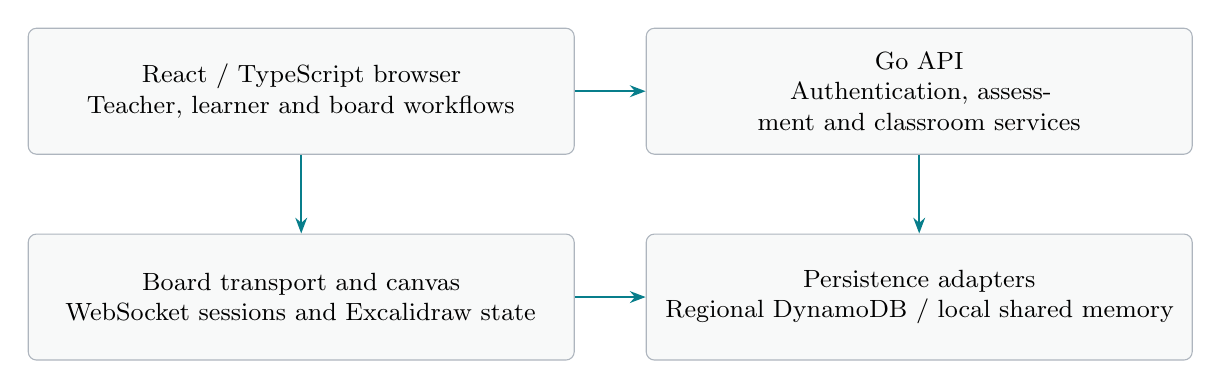
\begin{tikzpicture}[
box/.style={draw=ink!35,rounded corners=3pt,fill=ink!3,text width=67mm,align=center,minimum height=16mm,font=\small},
edge/.style={-{Stealth[length=2mm]},thick,draw=accent},
node distance=10mm and 9mm]
\node[box] (web) {React / TypeScript browser\\Teacher, learner and board workflows};
\node[box,right=of web] (api) {Go API\\Authentication, assessment and classroom services};
\node[box,below=of web] (board) {Board transport and canvas\\WebSocket sessions and Excalidraw state};
\node[box,below=of api] (store) {Persistence adapters\\Regional DynamoDB / local shared memory};
\draw[edge] (web) -- (api);
\draw[edge] (web) -- (board);
\draw[edge] (api) -- (store);
\draw[edge] (board) -- (store);
\end{tikzpicture}
\end{center}

\subsection{Correction boundaries}
The additional register starts after QF-200 and uses commit \texttt{e218e12} as its comparison point. Each entry describes a distinct trigger or user-facing outcome. Several entries share a component or root cause; a correction count is not a count of independent production incidents. The earlier CQ-001--CQ-120 audit and QF-001--QF-200 correction register are retained separately.

\begin{tabularx}{\linewidth}{@{}lrX@{}}
\toprule
Classification & Entries & Interpretation\\
\midrule
Behavioral corrections & 32 & Observable state, serialization, concurrency or recovery defects\\
Boundary hardening & 12 & Invalid transport or persisted data handled safely\\
Accessibility and polish & 56 & Clearer controls, readable content and recoverable interface states\\
\midrule
Total & 100 & Fixed entries QF-201--QF-300\\
\bottomrule
\end{tabularx}


\subsection{Assessment data contracts}
Authoring now preserves correct-answer index zero. Learner responses carry an explicit redaction decision instead of relying on numeric zero to omit a field. Submitted zero scores remain present in metadata. Model tests cover both answer indices and redaction; the teacher/learner browser journey checks preview visibility, learner answer-key omission and zero-score metadata.

\subsection{Board state and transport}
Peer registration is idempotent for a socket. Canceled broadcasts retain healthy participants, idle eviction rechecks recent traffic, and cleanup announces departures even after request cancellation. Snapshot application validates room identity, schema and revision. Explicit flush retains its originating writer identity while respecting its caller's cancellation.

Element copies isolate typed collections. Revision validation rejects invalid numeric ordering values, and equal-version conflicts use the Excalidraw nonce tie breaker. The browser validates socket envelopes, ignores disposed transport events and retains early deltas during lazy canvas loading. Large scenes are split by UTF-8 byte size beneath the default frame limit.

\subsection{User interaction and accessibility}
Account workflows preserve unsaved profile edits during background refresh and prevent edits that would be overwritten by a pending save. Password controls expose their state and disable unwanted keyboard correction. Repeated builder inputs and actions identify their question or draft. Dialogs scroll within constrained viewports, and empty/error states provide direct recovery actions.

These improvements preserve the established product styling. They focus on readable authored text, complete member identity, keyboard and assistive-technology context, and useful failure recovery.

\clearpage
\section{Verification and remaining limits}
\input{verification.tex}

\subsection{Regression focus}
Backend regressions cover serialization, peer registration, cancellation, heartbeat/eviction ordering, typed snapshot isolation, revision convergence, invalid persisted state and WebSocket request cleanup. Frontend regressions cover malformed socket messages, UTF-8 batching, old-socket events, constructor/send failures, shared token state, composed input groups, reviewed imports, profile editing and repeated authoring controls.

Existing broad tests remain in place. Expectations were updated only where intended behavior changed, such as rejecting frames from a detached session, validating a requested historical revision, normalized cache revisions and clearer action names.

\subsection{Operational boundary}
No live AWS deployment, production traffic exercise or external SMTP delivery is part of this batch. The default browser batching budget targets the configured default 64 KiB WebSocket limit; a custom lower deployment limit needs a matching client budget. An individual oversized element is reported to the user instead of being silently transmitted.

Earlier durability and authorization limitations remain tracked in the original audit. In particular, this batch does not claim durable acknowledgment for every drawing frame, complete offline conflict recovery, historical assessment receipts for every retake, or a complete resolution of the original backlog. The existing production-build chunk-size and route-export warnings remain.

\subsection{Project materials}
The full historical project report is \nolinkurl{output/pdf/continuum-project-quality-report-2026-10-23.pdf}. The preceding supplement is \nolinkurl{output/pdf/continuum-quality-fixes-2026-10-23.pdf}. The new JSON/Markdown register contains exact final source locations and SHA-256 source hashes. Editable LaTeX and its generator live under \nolinkurl{docs/quality-more-report/}.

\clearpage
\section{Additional correction register}
\small
% Generated by build_register.py; edit the DATA rows there.
\begin{minipage}{\linewidth}
\textbf{QF-201 --- Option zero disappears from authored JSON} {\scriptsize\color{accent}(Behavior)}\par
\textit{Trigger.} Save or preview a question whose correct option is A; the answer field was absent. \textit{Correction.} Encode zero explicitly for authoring and use a separate redaction flag on learner reads.\par
{\scriptsize\color{muted}\nolinkurl{internal/model/model.go}:93}\par
\end{minipage}\par\vspace{7pt}
\begin{minipage}{\linewidth}
\textbf{QF-202 --- Zero scores disappear from catalog metadata} {\scriptsize\color{accent}(Behavior)}\par
\textit{Trigger.} A submitted assessment scored zero serialized without its score field. \textit{Correction.} Keep numeric zero in the public metadata contract so submitted results stay distinguishable from missing data.\par
{\scriptsize\color{muted}\nolinkurl{internal/model/model.go}:123}\par
\end{minipage}\par\vspace{7pt}
\begin{minipage}{\linewidth}
\textbf{QF-203 --- Whitespace-only board names} {\scriptsize\color{accent}(Polish)}\par
\textit{Trigger.} Join with spaces as a display name; presence showed an empty-looking participant. \textit{Correction.} Trim names before applying the Guest fallback and length limit.\par
{\scriptsize\color{muted}\nolinkurl{internal/boards/manager.go}:128}\par
\end{minipage}\par\vspace{7pt}
\begin{minipage}{\linewidth}
\textbf{QF-204 --- Duplicate socket registration leaves phantom peers} {\scriptsize\color{accent}(Behavior)}\par
\textit{Trigger.} Connect the same socket twice; peer order contained it twice while the map retained one identity. \textit{Correction.} Return the existing peer ID without appending a second registration.\par
{\scriptsize\color{muted}\nolinkurl{internal/boards/manager.go}:168}\par
\end{minipage}\par\vspace{7pt}
\begin{minipage}{\linewidth}
\textbf{QF-205 --- Typed nil transports pass connection validation} {\scriptsize\color{accent}(Hardening)}\par
\textit{Trigger.} An integration passes a typed nil pointer as a socket; it was accepted and could panic on send. \textit{Correction.} Reject nil pointer, channel and interface transport values before registration.\par
{\scriptsize\color{muted}\nolinkurl{internal/boards/manager.go}:152}\par
\end{minipage}\par\vspace{7pt}
\begin{minipage}{\linewidth}
\textbf{QF-206 --- Non-comparable transport helpers panic} {\scriptsize\color{accent}(Hardening)}\par
\textit{Trigger.} Pass a slice or map to peer lookup helpers after room creation; map indexing could panic. \textit{Correction.} Apply the comparable-socket guard consistently to public peer operations and exclusions.\par
{\scriptsize\color{muted}\nolinkurl{internal/boards/manager.go}:618}\par
\end{minipage}\par\vspace{7pt}
\begin{minipage}{\linewidth}
\textbf{QF-207 --- Peerless rooms inflate active-room metrics} {\scriptsize\color{accent}(Behavior)}\par
\textit{Trigger.} Export or absorb a room with no connected peers; status counted it as active. \textit{Correction.} Count only rooms with at least one attached peer.\par
{\scriptsize\color{muted}\nolinkurl{internal/boards/manager.go}:361}\par
\end{minipage}\par\vspace{7pt}
\begin{minipage}{\linewidth}
\textbf{QF-208 --- Reset retains obsolete persistence errors} {\scriptsize\color{accent}(Behavior)}\par
\textit{Trigger.} Reset local board state after a failed save; LastPersistenceError still reported the old incident. \textit{Correction.} Clear asynchronous error state together with rooms and pending saves.\par
{\scriptsize\color{muted}\nolinkurl{internal/boards/manager.go}:374}\par
\end{minipage}\par\vspace{7pt}
\begin{minipage}{\linewidth}
\textbf{QF-209 --- Canceled broadcast removes healthy peers} {\scriptsize\color{accent}(Behavior)}\par
\textit{Trigger.} Cancel a broadcast context before or during delivery; healthy recipients were detached as transport failures. \textit{Correction.} Stop the broadcast on context cancellation without evicting recipients.\par
{\scriptsize\color{muted}\nolinkurl{internal/boards/manager.go}:486}\par
\end{minipage}\par\vspace{7pt}
\begin{minipage}{\linewidth}
\textbf{QF-210 --- Heartbeat races with idle eviction} {\scriptsize\color{accent}(Behavior)}\par
\textit{Trigger.} A peer sends fresh traffic after the sweep collects stale peers but before its turn is processed. \textit{Correction.} Recheck LastSeen under the room lock immediately before detaching the peer.\par
{\scriptsize\color{muted}\nolinkurl{internal/boards/manager.go}:665}\par
\end{minipage}\par\vspace{7pt}
\begin{minipage}{\linewidth}
\textbf{QF-211 --- Typed collections alias board snapshots} {\scriptsize\color{accent}(Behavior)}\par
\textit{Trigger.} Integrations pass typed point slices or nested maps; mutating input or returned snapshots could mutate live room state. \textit{Correction.} Recursively clone typed maps, slices and arrays while preserving their concrete types.\par
{\scriptsize\color{muted}\nolinkurl{internal/boards/manager.go}:626}\par
\end{minipage}\par\vspace{7pt}
\begin{minipage}{\linewidth}
\textbf{QF-212 --- Invalid element revisions enter ordering} {\scriptsize\color{accent}(Hardening)}\par
\textit{Trigger.} Negative, fractional, infinite or unsafe integer revisions could enter last-writer ordering and persistence. \textit{Correction.} Accept only finite, non-negative, safe integer revisions.\par
{\scriptsize\color{muted}\nolinkurl{internal/boards/manager.go}:697}\par
\end{minipage}\par\vspace{7pt}
\begin{minipage}{\linewidth}
\textbf{QF-213 --- Concurrent equal-version edits do not converge} {\scriptsize\color{accent}(Behavior)}\par
\textit{Trigger.} Two valid Excalidraw edits share a version but differ in versionNonce; arrival order determined the stored winner. \textit{Correction.} Use the lower nonce as the deterministic tie breaker, matching canvas reconciliation.\par
{\scriptsize\color{muted}\nolinkurl{internal/boards/persistence.go}:690}\par
\end{minipage}\par\vspace{7pt}
\begin{minipage}{\linewidth}
\textbf{QF-214 --- Unchanged repeated joins generate redundant announcements} {\scriptsize\color{accent}(Polish)}\par
\textit{Trigger.} Identity refresh or another join frame announced the same unchanged peer again. \textit{Correction.} Send init on rejoin while broadcasting presence only for first joins or actual identity changes.\par
{\scriptsize\color{muted}\nolinkurl{internal/boards/protocol.go}:127}\par
\end{minipage}\par\vspace{7pt}
\begin{minipage}{\linewidth}
\textbf{QF-215 --- Detached sessions can process new frames} {\scriptsize\color{accent}(Hardening)}\par
\textit{Trigger.} Call HandleFrame after Close or eviction; a stale session could still issue protocol operations. \textit{Correction.} Reject closed or no-longer-registered sessions before dispatch.\par
{\scriptsize\color{muted}\nolinkurl{internal/boards/protocol.go}:79}\par
\end{minipage}\par\vspace{7pt}
\begin{minipage}{\linewidth}
\textbf{QF-216 --- Canceled request suppresses peer departure} {\scriptsize\color{accent}(Behavior)}\par
\textit{Trigger.} Close a session using a canceled request context; remaining peers missed peer-left. \textit{Correction.} Detach once and announce departure using a cleanup context independent of request cancellation.\par
{\scriptsize\color{muted}\nolinkurl{internal/boards/protocol.go}:229}\par
\end{minipage}\par\vspace{7pt}
\begin{minipage}{\linewidth}
\textbf{QF-217 --- Canceled WebSocket requests keep blocking} {\scriptsize\color{accent}(Behavior)}\par
\textit{Trigger.} Cancel the HTTP request while ReadMessage waits for a silent client; the handler and peer remained alive. \textit{Correction.} Close the connection when its request context ends and stop the callback during normal cleanup.\par
{\scriptsize\color{muted}\nolinkurl{internal/boards/http.go}:122}\par
\end{minipage}\par\vspace{7pt}
\begin{minipage}{\linewidth}
\textbf{QF-218 --- Snapshots can load into the wrong room} {\scriptsize\color{accent}(Hardening)}\par
\textit{Trigger.} A backing adapter returns a snapshot with another room ID; Resume previously merged it. \textit{Correction.} Validate snapshot ownership before merging or restoring persisted content.\par
{\scriptsize\color{muted}\nolinkurl{internal/boards/persistence.go}:712}\par
\end{minipage}\par\vspace{7pt}
\begin{minipage}{\linewidth}
\textbf{QF-219 --- Unsupported snapshot schemas load silently} {\scriptsize\color{accent}(Hardening)}\par
\textit{Trigger.} A future or invalid schema revision was treated like the current format. \textit{Correction.} Accept the current schema and legacy zero only, returning an explicit error for unsupported schemas.\par
{\scriptsize\color{muted}\nolinkurl{internal/boards/persistence.go}:715}\par
\end{minipage}\par\vspace{7pt}
\begin{minipage}{\linewidth}
\textbf{QF-220 --- Invalid snapshot revisions damage room sequencing} {\scriptsize\color{accent}(Hardening)}\par
\textit{Trigger.} Negative or maximum int64 snapshot versions can corrupt the next room revision. \textit{Correction.} Reject invalid or immediately overflowing persisted revisions before applying them.\par
{\scriptsize\color{muted}\nolinkurl{internal/boards/persistence.go}:718}\par
\end{minipage}\par\vspace{7pt}
\begin{minipage}{\linewidth}
\textbf{QF-221 --- Canceled loads become cached successes} {\scriptsize\color{accent}(Behavior)}\par
\textit{Trigger.} A store ignores cancellation and returns successfully; Resume marked the room loaded anyway. \textit{Correction.} Check request cancellation after loading and leave the room eligible for a later successful resume.\par
{\scriptsize\color{muted}\nolinkurl{internal/boards/persistence.go}:297}\par
\end{minipage}\par\vspace{7pt}
\begin{minipage}{\linewidth}
\textbf{QF-222 --- Explicit flush ignores its caller cancellation} {\scriptsize\color{accent}(Behavior)}\par
\textit{Trigger.} A pending save retained its original writer context but also discarded a canceled flush caller. \textit{Correction.} Preserve writer identity values while honoring the flush caller's cancellation and deadline.\par
{\scriptsize\color{muted}\nolinkurl{internal/boards/persistence.go}:350}\par
\end{minipage}\par\vspace{7pt}
\begin{minipage}{\linewidth}
\textbf{QF-223 --- Restore accepts a different requested revision} {\scriptsize\color{accent}(Hardening)}\par
\textit{Trigger.} LoadVersion returns a valid snapshot for another revision; the manager restored it without checking. \textit{Correction.} Compare the returned revision with the requested version before touching the live room.\par
{\scriptsize\color{muted}\nolinkurl{internal/boards/persistence.go}:438}\par
\end{minipage}\par\vspace{7pt}
\begin{minipage}{\linewidth}
\textbf{QF-224 --- No-op permission changes create history} {\scriptsize\color{accent}(Polish)}\par
\textit{Trigger.} Repeat the current students-draw setting; it incremented versions and wrote another snapshot. \textit{Correction.} Return without persistence or broadcast when the setting is unchanged.\par
{\scriptsize\color{muted}\nolinkurl{internal/boards/permissions.go}:29}\par
\end{minipage}\par\vspace{7pt}
\begin{minipage}{\linewidth}
\textbf{QF-225 --- Admin token consumers disagree in one tab} {\scriptsize\color{accent}(Behavior)}\par
\textit{Trigger.} Save a token from one mounted hook; other consumers kept their previous local state. \textit{Correction.} Use one subscribed external store and notify every mounted consumer on writes.\par
{\scriptsize\color{muted}\nolinkurl{web/src/lib/admin-token.ts}:1}\par
\end{minipage}\par\vspace{7pt}
\begin{minipage}{\linewidth}
\textbf{QF-226 --- Admin token changes do not cross tabs} {\scriptsize\color{accent}(Behavior)}\par
\textit{Trigger.} Change or clear the token in another tab; existing consumers kept stale credentials. \textit{Correction.} Handle relevant local-storage events and full storage clears while ignoring other storage areas.\par
{\scriptsize\color{muted}\nolinkurl{web/src/lib/admin-token.ts}:15}\par
\end{minipage}\par\vspace{7pt}
\begin{minipage}{\linewidth}
\textbf{QF-227 --- Blocked storage loses shared ephemeral credentials} {\scriptsize\color{accent}(Behavior)}\par
\textit{Trigger.} A token write fails because storage is blocked; another component reading the token saw empty or old data. \textit{Correction.} Retain a shared in-memory fallback for the session and expose it consistently.\par
{\scriptsize\color{muted}\nolinkurl{web/src/lib/admin-token.ts}:23}\par
\end{minipage}\par\vspace{7pt}
\begin{minipage}{\linewidth}
\textbf{QF-228 --- Malformed socket envelopes crash consumers} {\scriptsize\color{accent}(Hardening)}\par
\textit{Trigger.} Valid JSON such as null, missing peers or non-array elements passed directly to callbacks. \textit{Correction.} Validate known message envelopes and ignore malformed frames before updating state.\par
{\scriptsize\color{muted}\nolinkurl{web/src/hooks/use-board-sync.ts}:39}\par
\end{minipage}\par\vspace{7pt}
\begin{minipage}{\linewidth}
\textbf{QF-229 --- Queued old-socket callbacks affect a new room} {\scriptsize\color{accent}(Behavior)}\par
\textit{Trigger.} A queued event arrives after room replacement or disposal; it could update the current callbacks and presence. \textit{Correction.} Check both disposal and socket identity before processing open, message and close events.\par
{\scriptsize\color{muted}\nolinkurl{web/src/hooks/use-board-sync.ts}:191}\par
\end{minipage}\par\vspace{7pt}
\begin{minipage}{\linewidth}
\textbf{QF-230 --- WebSocket constructor failures crash the page} {\scriptsize\color{accent}(Behavior)}\par
\textit{Trigger.} Browser policy or an invalid connection environment throws synchronously during socket construction. \textit{Correction.} Expose an unavailable state with a recoverable error instead of escaping the effect.\par
{\scriptsize\color{muted}\nolinkurl{web/src/hooks/use-board-sync.ts}:184}\par
\end{minipage}\par\vspace{7pt}
\begin{minipage}{\linewidth}
\textbf{QF-231 --- Synchronous send errors lose a drawing batch} {\scriptsize\color{accent}(Behavior)}\par
\textit{Trigger.} A socket closes between readyState checking and send; the exception escaped without buffering work. \textit{Correction.} Catch send failure, close the failed transport and retain the element batch for reconnect.\par
{\scriptsize\color{muted}\nolinkurl{web/src/hooks/use-board-sync.ts}:142}\par
\end{minipage}\par\vspace{7pt}
\begin{minipage}{\linewidth}
\textbf{QF-232 --- Disconnected presence remains visible} {\scriptsize\color{accent}(Polish)}\par
\textit{Trigger.} A connection closes but the participant list and self ID stayed visible until another init. \textit{Correction.} Clear disconnected presence immediately while reconnecting.\par
{\scriptsize\color{muted}\nolinkurl{web/src/hooks/use-board-sync.ts}:276}\par
\end{minipage}\par\vspace{7pt}
\begin{minipage}{\linewidth}
\textbf{QF-233 --- Online recovery waits for exponential backoff} {\scriptsize\color{accent}(Polish)}\par
\textit{Trigger.} The browser regains connectivity while a reconnect timer is waiting. \textit{Correction.} Attempt reconnect immediately on the online event and remove the listener during cleanup.\par
{\scriptsize\color{muted}\nolinkurl{web/src/hooks/use-board-sync.ts}:313}\par
\end{minipage}\par\vspace{7pt}
\begin{minipage}{\linewidth}
\textbf{QF-234 --- Large drawing batches exceed the frame limit} {\scriptsize\color{accent}(Behavior)}\par
\textit{Trigger.} A normal gesture produces a multi-element batch larger than the server's 64 KiB limit and disconnects. \textit{Correction.} Split by encoded UTF-8 size with envelope headroom and explain an individually oversized element.\par
{\scriptsize\color{muted}\nolinkurl{web/src/hooks/use-board-sync.ts}:81}\par
\end{minipage}\par\vspace{7pt}
\begin{minipage}{\linewidth}
\textbf{QF-235 --- One corrupt cache row discards the local scene} {\scriptsize\color{accent}(Hardening)}\par
\textit{Trigger.} A local snapshot mixes valid elements with null or malformed rows; the broad catch discarded everything. \textit{Correction.} Validate rows individually and recover the valid subset with normalized revision defaults.\par
{\scriptsize\color{muted}\nolinkurl{web/src/components/board/board-canvas.tsx}:60}\par
\end{minipage}\par\vspace{7pt}
\begin{minipage}{\linewidth}
\textbf{QF-236 --- Duplicate cached IDs retain stale revisions} {\scriptsize\color{accent}(Behavior)}\par
\textit{Trigger.} A cached scene has repeated IDs in a different revision order; the last array row could overwrite newer state. \textit{Correction.} Keep the newest element revision and deterministic nonce winner for each ID.\par
{\scriptsize\color{muted}\nolinkurl{web/src/lib/board-elements.ts}:14}\par
\end{minipage}\par\vspace{7pt}
\begin{minipage}{\linewidth}
\textbf{QF-237 --- Board deltas arrive before the lazy canvas exists} {\scriptsize\color{accent}(Behavior)}\par
\textit{Trigger.} An elements frame arrives after init while the canvas module is still loading; the optional callback dropped it. \textit{Correction.} Merge early deltas into the pending remote snapshot until the canvas can consume them.\par
{\scriptsize\color{muted}\nolinkurl{web/src/routes/board.$roomId.tsx}:86}\par
\end{minipage}\par\vspace{7pt}
\begin{minipage}{\linewidth}
\textbf{QF-238 --- An empty room still opens a socket} {\scriptsize\color{accent}(Hardening)}\par
\textit{Trigger.} A route normalizes to an empty room code; the error view appeared while its hook still connected. \textit{Correction.} Disable realtime transport for an empty room identifier.\par
{\scriptsize\color{muted}\nolinkurl{web/src/routes/board.$roomId.tsx}:95}\par
\end{minipage}\par\vspace{7pt}
\begin{minipage}{\linewidth}
\textbf{QF-239 --- Repeated export clicks create overlapping downloads} {\scriptsize\color{accent}(Polish)}\par
\textit{Trigger.} Click Export repeatedly while the persistence request is pending. \textit{Correction.} Use a synchronous export lock and a visible exporting state until completion.\par
{\scriptsize\color{muted}\nolinkurl{web/src/routes/board.$roomId.tsx}:142}\par
\end{minipage}\par\vspace{7pt}
\begin{minipage}{\linewidth}
\textbf{QF-240 --- Board JSON downloads revoke URLs immediately} {\scriptsize\color{accent}(Behavior)}\par
\textit{Trigger.} The board export clicked an unattached anchor and immediately revoked its blob URL. \textit{Correction.} Reuse the attached-anchor download helper with delayed object-URL cleanup.\par
{\scriptsize\color{muted}\nolinkurl{web/src/routes/board.$roomId.tsx}:172}\par
\end{minipage}\par\vspace{7pt}
\begin{minipage}{\linewidth}
\textbf{QF-241 --- Board download failures have no actionable feedback} {\scriptsize\color{accent}(Polish)}\par
\textit{Trigger.} Blob URL creation or a download operation throws; the async event handler rejected without guidance. \textit{Correction.} Catch download errors, release the pending state and show a retryable failure message.\par
{\scriptsize\color{muted}\nolinkurl{web/src/routes/board.$roomId.tsx}:179}\par
\end{minipage}\par\vspace{7pt}
\begin{minipage}{\linewidth}
\textbf{QF-242 --- Constructor failure leaves no retry control} {\scriptsize\color{accent}(Polish)}\par
\textit{Trigger.} Realtime is configured but socket construction fails; the unavailable state had no Retry now button. \textit{Correction.} Expose manual retry for recoverable unavailable connections as well as reconnecting ones.\par
{\scriptsize\color{muted}\nolinkurl{web/src/routes/board.$roomId.tsx}:212}\par
\end{minipage}\par\vspace{7pt}
\begin{minipage}{\linewidth}
\textbf{QF-243 --- Room-code button lacks an explicit copy action} {\scriptsize\color{accent}(Polish)}\par
\textit{Trigger.} The toolbar button's accessible name was only the code, leaving its purpose unclear. \textit{Correction.} Name the control with the copy action and complete room code.\par
{\scriptsize\color{muted}\nolinkurl{web/src/routes/board.$roomId.tsx}:242}\par
\end{minipage}\par\vspace{7pt}
\begin{minipage}{\linewidth}
\textbf{QF-244 --- Heartbeat send exceptions escape the timer} {\scriptsize\color{accent}(Behavior)}\par
\textit{Trigger.} The socket closes during an interval heartbeat; send could throw outside the transport recovery path. \textit{Correction.} Catch heartbeat send failure and close the transport to enter reconnect handling.\par
{\scriptsize\color{muted}\nolinkurl{web/src/hooks/use-board-sync.ts}:207}\par
\end{minipage}\par\vspace{7pt}
\begin{minipage}{\linewidth}
\textbf{QF-245 --- Late history restore replaces another room} {\scriptsize\color{accent}(Behavior)}\par
\textit{Trigger.} Change rooms or user identity while restore is pending; its late response applied through the current callback. \textit{Correction.} Capture the requested room and user scope and ignore a response after either changes.\par
{\scriptsize\color{muted}\nolinkurl{web/src/components/board/board-history-dialog.tsx}:90}\par
\end{minipage}\par\vspace{7pt}
\begin{minipage}{\linewidth}
\textbf{QF-246 --- History restore controls are indistinguishable} {\scriptsize\color{accent}(Polish)}\par
\textit{Trigger.} A screen-reader button list contains multiple controls all named Restore. \textit{Correction.} Include the target revision in each restore button's accessible name.\par
{\scriptsize\color{muted}\nolinkurl{web/src/components/board/board-history-dialog.tsx}:104}\par
\end{minipage}\par\vspace{7pt}
\begin{minipage}{\linewidth}
\textbf{QF-247 --- Malformed history timestamps show Invalid Date} {\scriptsize\color{accent}(Polish)}\par
\textit{Trigger.} A history adapter returns an invalid saved\_at string. \textit{Correction.} Display a clear unavailable-time fallback instead of rendering Invalid Date.\par
{\scriptsize\color{muted}\nolinkurl{web/src/components/board/board-history-dialog.tsx}:80}\par
\end{minipage}\par\vspace{7pt}
\begin{minipage}{\linewidth}
\textbf{QF-248 --- Standard dialogs exceed short viewports} {\scriptsize\color{accent}(Polish)}\par
\textit{Trigger.} Open a tall dialog with a short window or virtual keyboard; top or bottom content can be unreachable. \textit{Correction.} Bound popup height to the dynamic viewport and allow internal vertical scrolling.\par
{\scriptsize\color{muted}\nolinkurl{web/src/components/ui/dialog.tsx}:56}\par
\end{minipage}\par\vspace{7pt}
\begin{minipage}{\linewidth}
\textbf{QF-249 --- Dialog headings overlap the close control} {\scriptsize\color{accent}(Polish)}\par
\textit{Trigger.} A long dialog title reaches the top-right close button. \textit{Correction.} Reserve header space for the close control.\par
{\scriptsize\color{muted}\nolinkurl{web/src/components/ui/dialog.tsx}:86}\par
\end{minipage}\par\vspace{7pt}
\begin{minipage}{\linewidth}
\textbf{QF-250 --- Confirmations overflow very narrow screens} {\scriptsize\color{accent}(Polish)}\par
\textit{Trigger.} The alert popup's full width and fixed maximum can reach viewport edges at small widths. \textit{Correction.} Keep a viewport-relative width with consistent outer margins.\par
{\scriptsize\color{muted}\nolinkurl{web/src/components/ui/alert-dialog.tsx}:53}\par
\end{minipage}\par\vspace{7pt}
\begin{minipage}{\linewidth}
\textbf{QF-251 --- Long confirmations exceed the visible height} {\scriptsize\color{accent}(Polish)}\par
\textit{Trigger.} A confirmation has long text or an error on a short screen. \textit{Correction.} Bound its height and scroll its contents so actions remain reachable.\par
{\scriptsize\color{muted}\nolinkurl{web/src/components/ui/alert-dialog.tsx}:53}\par
\end{minipage}\par\vspace{7pt}
\begin{minipage}{\linewidth}
\textbf{QF-252 --- Unbroken names overflow confirmation titles} {\scriptsize\color{accent}(Polish)}\par
\textit{Trigger.} An item title contains a long token without spaces. \textit{Correction.} Allow long confirmation titles to wrap anywhere within the popup.\par
{\scriptsize\color{muted}\nolinkurl{web/src/components/ui/alert-dialog.tsx}:118}\par
\end{minipage}\par\vspace{7pt}
\begin{minipage}{\linewidth}
\textbf{QF-253 --- Pending confirmations are not communicated as busy} {\scriptsize\color{accent}(Polish)}\par
\textit{Trigger.} A destructive request waits while controls are disabled, without exposing busy state. \textit{Correction.} Mark the dialog busy and announce the changing confirmation action label politely.\par
{\scriptsize\color{muted}\nolinkurl{web/src/components/confirm-action.tsx}:61}\par
\end{minipage}\par\vspace{7pt}
\begin{minipage}{\linewidth}
\textbf{QF-254 --- Input-group addons do not focus textareas} {\scriptsize\color{accent}(Behavior)}\par
\textit{Trigger.} Click a text addon next to an InputGroupTextarea; the helper searched only for input. \textit{Correction.} Focus either supported editable control.\par
{\scriptsize\color{muted}\nolinkurl{web/src/components/ui/input-group.tsx}:64}\par
\end{minipage}\par\vspace{7pt}
\begin{minipage}{\linewidth}
\textbf{QF-255 --- Custom addon click handlers suppress built-in focus} {\scriptsize\color{accent}(Behavior)}\par
\textit{Trigger.} Passing onClick replaced the internal focus handler through prop spreading. \textit{Correction.} Compose the supplied callback with default focus behavior and respect preventDefault.\par
{\scriptsize\color{muted}\nolinkurl{web/src/components/ui/input-group.tsx}:58}\par
\end{minipage}\par\vspace{7pt}
\begin{minipage}{\linewidth}
\textbf{QF-256 --- Home catalog failures require a page refresh} {\scriptsize\color{accent}(Polish)}\par
\textit{Trigger.} The assessment catalog fails but the error state offers only explanatory text. \textit{Correction.} Add a catalog retry control that refetches the failed query.\par
{\scriptsize\color{muted}\nolinkurl{web/src/routes/index.tsx}:257}\par
\end{minipage}\par\vspace{7pt}
\begin{minipage}{\linewidth}
\textbf{QF-257 --- Empty assessment searches lack a reset action} {\scriptsize\color{accent}(Polish)}\par
\textit{Trigger.} Search and class/status filters produce zero results; recovery requires clearing several controls manually. \textit{Correction.} Reset search, status and classroom filters from the empty state.\par
{\scriptsize\color{muted}\nolinkurl{web/src/routes/index.tsx}:351}\par
\end{minipage}\par\vspace{7pt}
\begin{minipage}{\linewidth}
\textbf{QF-258 --- Empty room searches lack a reset action} {\scriptsize\color{accent}(Polish)}\par
\textit{Trigger.} A room filter yields no results with only text suggesting that it be cleared. \textit{Correction.} Provide a clear-filter action in the empty state.\par
{\scriptsize\color{muted}\nolinkurl{web/src/routes/board.index.tsx}:275}\par
\end{minipage}\par\vspace{7pt}
\begin{minipage}{\linewidth}
\textbf{QF-259 --- Filtered assessment counts are silent} {\scriptsize\color{accent}(Polish)}\par
\textit{Trigger.} Change filters while using assistive technology; the changing badge is not announced. \textit{Correction.} Expose the count as a named polite status.\par
{\scriptsize\color{muted}\nolinkurl{web/src/routes/index.tsx}:218}\par
\end{minipage}\par\vspace{7pt}
\begin{minipage}{\linewidth}
\textbf{QF-260 --- IME confirmation can submit authentication} {\scriptsize\color{accent}(Behavior)}\par
\textit{Trigger.} Press Enter to finish composing text in an authentication field; it also submits credentials. \textit{Correction.} Ignore Enter submission while the browser reports active composition.\par
{\scriptsize\color{muted}\nolinkurl{web/src/routes/login.tsx}:401}\par
\end{minipage}\par\vspace{7pt}
\begin{minipage}{\linewidth}
\textbf{QF-261 --- Recovery email fields enable unwanted typing assistance} {\scriptsize\color{accent}(Polish)}\par
\textit{Trigger.} On mobile, recovery email entry can receive capitalization or spellchecking behavior. \textit{Correction.} Disable capitalization, autocorrection and spellchecking for the recovery address.\par
{\scriptsize\color{muted}\nolinkurl{web/src/routes/login.tsx}:299}\par
\end{minipage}\par\vspace{7pt}
\begin{minipage}{\linewidth}
\textbf{QF-262 --- Password visibility controls do not expose state} {\scriptsize\color{accent}(Polish)}\par
\textit{Trigger.} Toggle password visibility in authentication or settings; only the label changes. \textit{Correction.} Expose the pressed state on all password visibility controls.\par
{\scriptsize\color{muted}\nolinkurl{web/src/routes/login.tsx}:462}\par
\end{minipage}\par\vspace{7pt}
\begin{minipage}{\linewidth}
\textbf{QF-263 --- Visible passwords can receive text autocorrection} {\scriptsize\color{accent}(Polish)}\par
\textit{Trigger.} Show a password as text on mobile; default keyboard assistance can modify its contents. \textit{Correction.} Disable capitalization, correction and spellchecking on password inputs in both account flows.\par
{\scriptsize\color{muted}\nolinkurl{web/src/routes/login.tsx}:245}\par
\end{minipage}\par\vspace{7pt}
\begin{minipage}{\linewidth}
\textbf{QF-264 --- Profile edits made during save are overwritten} {\scriptsize\color{accent}(Behavior)}\par
\textit{Trigger.} Type another display name while an earlier profile update is pending; the response replaces that new edit. \textit{Correction.} Disable the profile input for its pending write.\par
{\scriptsize\color{muted}\nolinkurl{web/src/routes/settings.tsx}:172}\par
\end{minipage}\par\vspace{7pt}
\begin{minipage}{\linewidth}
\textbf{QF-265 --- New credentials typed during a password change are erased} {\scriptsize\color{accent}(Behavior)}\par
\textit{Trigger.} Edit password fields while the mutation waits; successful cleanup clears those newly typed values. \textit{Correction.} Disable both password inputs and visibility controls while the request is pending.\par
{\scriptsize\color{muted}\nolinkurl{web/src/routes/settings.tsx}:236}\par
\end{minipage}\par\vspace{7pt}
\begin{minipage}{\linewidth}
\textbf{QF-266 --- Overlong profile names fail only after submission} {\scriptsize\color{accent}(Polish)}\par
\textit{Trigger.} Enter more than the server's 60-character profile limit with no field guidance. \textit{Correction.} Validate character count locally, explain the limit and disable invalid saves.\par
{\scriptsize\color{muted}\nolinkurl{web/src/routes/settings.tsx}:60}\par
\end{minipage}\par\vspace{7pt}
\begin{minipage}{\linewidth}
\textbf{QF-267 --- Background profile refresh destroys unsaved names} {\scriptsize\color{accent}(Behavior)}\par
\textit{Trigger.} A same-user identity refresh updates the canonical name while a local profile edit is in progress. \textit{Correction.} Update pristine values on refresh and preserve an independently edited local name.\par
{\scriptsize\color{muted}\nolinkurl{web/src/routes/settings.tsx}:56}\par
\end{minipage}\par\vspace{7pt}
\begin{minipage}{\linewidth}
\textbf{QF-268 --- Password instructions disagree with byte-based validation} {\scriptsize\color{accent}(Polish)}\par
\textit{Trigger.} The settings description promises eight characters while the actual policy measures UTF-8 bytes. \textit{Correction.} Explain the 8–72-byte range and how non-ASCII text affects it.\par
{\scriptsize\color{muted}\nolinkurl{web/src/routes/settings.tsx}:223}\par
\end{minipage}\par\vspace{7pt}
\begin{minipage}{\linewidth}
\textbf{QF-269 --- Settings password validation lacks input semantics} {\scriptsize\color{accent}(Polish)}\par
\textit{Trigger.} A password field is visibly invalid but does not expose aria-invalid or its help text association. \textit{Correction.} Connect the live validation message to the input and expose its invalid state.\par
{\scriptsize\color{muted}\nolinkurl{web/src/routes/settings.tsx}:280}\par
\end{minipage}\par\vspace{7pt}
\begin{minipage}{\linewidth}
\textbf{QF-270 --- Authentication validation is only visual} {\scriptsize\color{accent}(Polish)}\par
\textit{Trigger.} Registration and reset fields show invalid styling without equivalent input semantics. \textit{Correction.} Expose invalid field states and associate password guidance with the relevant inputs.\par
{\scriptsize\color{muted}\nolinkurl{web/src/routes/login.tsx}:433}\par
\end{minipage}\par\vspace{7pt}
\begin{minipage}{\linewidth}
\textbf{QF-271 --- Builder validation is only visual} {\scriptsize\color{accent}(Polish)}\par
\textit{Trigger.} Invalid time, duration or attempt settings color their groups without exposing input-level errors. \textit{Correction.} Add invalid state and associated guidance to the affected question-builder controls.\par
{\scriptsize\color{muted}\nolinkurl{web/src/components/teacher/quiz-builder.tsx}:975}\par
\end{minipage}\par\vspace{7pt}
\begin{minipage}{\linewidth}
\textbf{QF-272 --- Repeated prompts lack question context} {\scriptsize\color{accent}(Polish)}\par
\textit{Trigger.} A teacher navigates text fields for several questions; every prompt is named Prompt. \textit{Correction.} Include the question number in each prompt's accessible name.\par
{\scriptsize\color{muted}\nolinkurl{web/src/components/teacher/quiz-builder.tsx}:1425}\par
\end{minipage}\par\vspace{7pt}
\begin{minipage}{\linewidth}
\textbf{QF-273 --- Correct-answer controls hide their selected state} {\scriptsize\color{accent}(Polish)}\par
\textit{Trigger.} The current answer is conveyed through a visual badge and button color only. \textit{Correction.} Expose the selected correct option with aria-pressed.\par
{\scriptsize\color{muted}\nolinkurl{web/src/components/teacher/quiz-builder.tsx}:1459}\par
\end{minipage}\par\vspace{7pt}
\begin{minipage}{\linewidth}
\textbf{QF-274 --- Repeated option controls lack question context} {\scriptsize\color{accent}(Polish)}\par
\textit{Trigger.} Option A and answer-selection controls repeat across multiple question cards. \textit{Correction.} Include the question number in option input and correct-answer action names.\par
{\scriptsize\color{muted}\nolinkurl{web/src/components/teacher/quiz-builder.tsx}:1447}\par
\end{minipage}\par\vspace{7pt}
\begin{minipage}{\linewidth}
\textbf{QF-275 --- Repeated feedback fields lack question context} {\scriptsize\color{accent}(Polish)}\par
\textit{Trigger.} Several feedback inputs have the same accessible name. \textit{Correction.} Identify each feedback field by question number.\par
{\scriptsize\color{muted}\nolinkurl{web/src/components/teacher/quiz-builder.tsx}:1530}\par
\end{minipage}\par\vspace{7pt}
\begin{minipage}{\linewidth}
\textbf{QF-276 --- Repeated scoring fields lack question context} {\scriptsize\color{accent}(Polish)}\par
\textit{Trigger.} Several point inputs have the same accessible name. \textit{Correction.} Identify each points field by question number.\par
{\scriptsize\color{muted}\nolinkurl{web/src/components/teacher/quiz-builder.tsx}:1509}\par
\end{minipage}\par\vspace{7pt}
\begin{minipage}{\linewidth}
\textbf{QF-277 --- Bank-save actions lack question context} {\scriptsize\color{accent}(Polish)}\par
\textit{Trigger.} A list of builder buttons contains several controls named Bank. \textit{Correction.} Name each save-to-bank action with its question number and purpose.\par
{\scriptsize\color{muted}\nolinkurl{web/src/components/teacher/quiz-builder.tsx}:1411}\par
\end{minipage}\par\vspace{7pt}
\begin{minipage}{\linewidth}
\textbf{QF-278 --- Add-option actions lack question context} {\scriptsize\color{accent}(Polish)}\par
\textit{Trigger.} Multiple question cards expose identical Add option controls. \textit{Correction.} Include the receiving question number in each add-option action.\par
{\scriptsize\color{muted}\nolinkurl{web/src/components/teacher/quiz-builder.tsx}:1496}\par
\end{minipage}\par\vspace{7pt}
\begin{minipage}{\linewidth}
\textbf{QF-279 --- Remove-option actions lack question context} {\scriptsize\color{accent}(Polish)}\par
\textit{Trigger.} A screen-reader action list repeats Remove option A across question cards. \textit{Correction.} Identify both the question and option being removed.\par
{\scriptsize\color{muted}\nolinkurl{web/src/components/teacher/quiz-builder.tsx}:1479}\par
\end{minipage}\par\vspace{7pt}
\begin{minipage}{\linewidth}
\textbf{QF-280 --- Local draft actions are indistinguishable} {\scriptsize\color{accent}(Polish)}\par
\textit{Trigger.} Several local rows expose identical Load controls. \textit{Correction.} Include the local draft title and storage context in the action name.\par
{\scriptsize\color{muted}\nolinkurl{web/src/components/teacher/quiz-builder.tsx}:1117}\par
\end{minipage}\par\vspace{7pt}
\begin{minipage}{\linewidth}
\textbf{QF-281 --- Workspace draft actions are indistinguishable} {\scriptsize\color{accent}(Polish)}\par
\textit{Trigger.} Several remote rows expose identical Load controls. \textit{Correction.} Include the workspace draft title and storage context in the action name.\par
{\scriptsize\color{muted}\nolinkurl{web/src/components/teacher/quiz-builder.tsx}:1202}\par
\end{minipage}\par\vspace{7pt}
\begin{minipage}{\linewidth}
\textbf{QF-282 --- Question-bank reuse actions are indistinguishable} {\scriptsize\color{accent}(Polish)}\par
\textit{Trigger.} Each bank row exposes a button named Use, without naming its question. \textit{Correction.} Include the question text in the reuse action name.\par
{\scriptsize\color{muted}\nolinkurl{web/src/components/teacher/quiz-builder.tsx}:1300}\par
\end{minipage}\par\vspace{7pt}
\begin{minipage}{\linewidth}
\textbf{QF-283 --- Draft list titles are permanently truncated} {\scriptsize\color{accent}(Polish)}\par
\textit{Trigger.} Long local or workspace draft titles cannot be distinguished visually in their rows. \textit{Correction.} Wrap full draft titles, including authored line breaks.\par
{\scriptsize\color{muted}\nolinkurl{web/src/components/teacher/quiz-builder.tsx}:1106}\par
\end{minipage}\par\vspace{7pt}
\begin{minipage}{\linewidth}
\textbf{QF-284 --- Question-bank prompts hide distinguishing content} {\scriptsize\color{accent}(Polish)}\par
\textit{Trigger.} Long bank prompts are truncated, concealing differences between similar questions. \textit{Correction.} Wrap complete question text and preserve authored line breaks.\par
{\scriptsize\color{muted}\nolinkurl{web/src/components/teacher/quiz-builder.tsx}:1292}\par
\end{minipage}\par\vspace{7pt}
\begin{minipage}{\linewidth}
\textbf{QF-285 --- Workspace draft failures have no retry control} {\scriptsize\color{accent}(Polish)}\par
\textit{Trigger.} Loading the remote drafts fails; only an error sentence is available. \textit{Correction.} Add a retry action while keeping local drafts available.\par
{\scriptsize\color{muted}\nolinkurl{web/src/components/teacher/quiz-builder.tsx}:1254}\par
\end{minipage}\par\vspace{7pt}
\begin{minipage}{\linewidth}
\textbf{QF-286 --- Missing builder assignments appear unassigned} {\scriptsize\color{accent}(Polish)}\par
\textit{Trigger.} Load a draft assigned to a class outside the current classroom list; the select has no matching option. \textit{Correction.} Keep an explicit unavailable-assignment option for the selected classroom ID.\par
{\scriptsize\color{muted}\nolinkurl{web/src/components/teacher/quiz-builder.tsx}:926}\par
\end{minipage}\par\vspace{7pt}
\begin{minipage}{\linewidth}
\textbf{QF-287 --- Duration zero conflicts with the builder's native minimum} {\scriptsize\color{accent}(Polish)}\par
\textit{Trigger.} The backend supports zero for unlimited duration but the builder sets its numeric minimum to one. \textit{Correction.} Align the numeric minimum and guidance with the supported zero value.\par
{\scriptsize\color{muted}\nolinkurl{web/src/components/teacher/quiz-builder.tsx}:1003}\par
\end{minipage}\par\vspace{7pt}
\begin{minipage}{\linewidth}
\textbf{QF-288 --- One invalid date can pass publish readiness} {\scriptsize\color{accent}(Hardening)}\par
\textit{Trigger.} Only one time boundary is invalid; the previous window expression short-circuits as valid. \textit{Correction.} Validate each supplied date independently before enabling publication.\par
{\scriptsize\color{muted}\nolinkurl{web/src/components/teacher/quiz-builder.tsx}:796}\par
\end{minipage}\par\vspace{7pt}
\begin{minipage}{\linewidth}
\textbf{QF-289 --- Import preview collapses multiline prompts} {\scriptsize\color{accent}(Polish)}\par
\textit{Trigger.} A question prompt contains authored line breaks; preview collapses them. \textit{Correction.} Preserve prompt whitespace and wrap long words during review.\par
{\scriptsize\color{muted}\nolinkurl{web/src/components/teacher/question-import.tsx}:147}\par
\end{minipage}\par\vspace{7pt}
\begin{minipage}{\linewidth}
\textbf{QF-290 --- Import preview merges choices into ambiguous text} {\scriptsize\color{accent}(Polish)}\par
\textit{Trigger.} Options contain separators or line breaks; a joined paragraph obscures choice boundaries. \textit{Correction.} Render each option as a separate ordered list item with its answer marker.\par
{\scriptsize\color{muted}\nolinkurl{web/src/components/teacher/question-import.tsx}:149}\par
\end{minipage}\par\vspace{7pt}
\begin{minipage}{\linewidth}
\textbf{QF-291 --- Import preview collapses feedback formatting} {\scriptsize\color{accent}(Polish)}\par
\textit{Trigger.} A feedback explanation contains multiple lines or a long token. \textit{Correction.} Preserve line breaks and wrap feedback within the preview.\par
{\scriptsize\color{muted}\nolinkurl{web/src/components/teacher/question-import.tsx}:166}\par
\end{minipage}\par\vspace{7pt}
\begin{minipage}{\linewidth}
\textbf{QF-292 --- Import format instructions are disconnected from inputs} {\scriptsize\color{accent}(Polish)}\par
\textit{Trigger.} Assistive technology reaches the format or source field without its required data-shape guidance. \textit{Correction.} Associate both controls with the format-specific instructions.\par
{\scriptsize\color{muted}\nolinkurl{web/src/components/teacher/question-import.tsx}:65}\par
\end{minipage}\par\vspace{7pt}
\begin{minipage}{\linewidth}
\textbf{QF-293 --- One reviewed import can be inserted twice} {\scriptsize\color{accent}(Behavior)}\par
\textit{Trigger.} Two activations occur before the cleared preview rerenders; the same reviewed batch is appended twice. \textit{Correction.} Guard insertion synchronously and reset the guard for a new preview.\par
{\scriptsize\color{muted}\nolinkurl{web/src/components/teacher/question-import.tsx}:43}\par
\end{minipage}\par\vspace{7pt}
\begin{minipage}{\linewidth}
\textbf{QF-294 --- Workspace draft loading has no announced status} {\scriptsize\color{accent}(Polish)}\par
\textit{Trigger.} The remote draft section shows only a skeleton while loading. \textit{Correction.} Give the loading region a named status for assistive technology.\par
{\scriptsize\color{muted}\nolinkurl{web/src/components/teacher/quiz-builder.tsx}:1156}\par
\end{minipage}\par\vspace{7pt}
\begin{minipage}{\linewidth}
\textbf{QF-295 --- Question-bank loading has no announced status} {\scriptsize\color{accent}(Polish)}\par
\textit{Trigger.} The empty local bank waits for its remote query with only a skeleton. \textit{Correction.} Give the bank loading region a named status.\par
{\scriptsize\color{muted}\nolinkurl{web/src/components/teacher/quiz-builder.tsx}:1283}\par
\end{minipage}\par\vspace{7pt}
\begin{minipage}{\linewidth}
\textbf{QF-296 --- The not-found page lacks a main landmark and heading} {\scriptsize\color{accent}(Polish)}\par
\textit{Trigger.} A user reaches an unknown route and cannot find a page heading or main landmark. \textit{Correction.} Use a main landmark and a real level-one 404 heading.\par
{\scriptsize\color{muted}\nolinkurl{web/src/routes/__root.tsx}:62}\par
\end{minipage}\par\vspace{7pt}
\begin{minipage}{\linewidth}
\textbf{QF-297 --- The rendering-error page lacks announced structure} {\scriptsize\color{accent}(Polish)}\par
\textit{Trigger.} A route rendering error shows plain paragraphs without alert semantics or a heading. \textit{Correction.} Use an alerting main region and a level-one error heading.\par
{\scriptsize\color{muted}\nolinkurl{web/src/routes/__root.tsx}:76}\par
\end{minipage}\par\vspace{7pt}
\begin{minipage}{\linewidth}
\textbf{QF-298 --- Header ellipsis hides complete page context} {\scriptsize\color{accent}(Polish)}\par
\textit{Trigger.} A narrow header truncates the title and description with no pointer-accessible disclosure. \textit{Correction.} Expose the full title and description through their title attributes.\par
{\scriptsize\color{muted}\nolinkurl{web/src/components/layout/app-shell.tsx}:44}\par
\end{minipage}\par\vspace{7pt}
\begin{minipage}{\linewidth}
\textbf{QF-299 --- Roster rows hide full member identities} {\scriptsize\color{accent}(Polish)}\par
\textit{Trigger.} Names and emails in roster rows are ellipsized, concealing the distinguishing part. \textit{Correction.} Wrap complete member names and email addresses within their table cells.\par
{\scriptsize\color{muted}\nolinkurl{web/src/components/classroom-dashboard-real.tsx}:691}\par
\end{minipage}\par\vspace{7pt}
\begin{minipage}{\linewidth}
\textbf{QF-300 --- Invitation cards hide full recipient identities} {\scriptsize\color{accent}(Polish)}\par
\textit{Trigger.} Long recipient names and addresses are truncated in pending invitation cards. \textit{Correction.} Wrap full recipient details so teachers can verify the invitation destination.\par
{\scriptsize\color{muted}\nolinkurl{web/src/components/classroom-dashboard-real.tsx}:873}\par
\end{minipage}\par\vspace{7pt}
\end{document}
